% This is samplepaper.tex, a sample chapter demonstrating the
% LLNCS macro package for Springer Computer Science proceedings;
% Version 2.20 of 2017/10/04
%
\documentclass[runningheads]{llncs}
%
\usepackage{graphicx}
\usepackage[acronym]{glossaries}
\usepackage{mathtools}
\usepackage{amssymb}
\graphicspath{ {./images/} }
\newacronym{ann}{ANN}{Artificial Neural Network}
\newacronym{anns}{ANNs}{Artificial Neural Networks}
% Used for displaying a sample figure. If possible, figure files should
% be included in EPS format.
%
% If you use the hyperref package, please uncomment the following line
% to display URLs in blue roman font according to Springer's eBook style:
% \renewcommand\UrlFont{\color{blue}\rmfamily}

\begin{document}
%
\title{Neural networks and Deep Learning \thanks{Supported by organization x.}}
%
%\titlerunning{Abbreviated paper title}
% If the paper title is too long for the running head, you can set
% an abbreviated paper title here
%
\author{Mohamed Hesham Ibrahim Abdalla\inst{1}\orcidID{0000-1111-2222-3333} \and
Second Author\inst{1}\orcidID{1111-2222-3333-4444} \and
Third Author\inst{1}\orcidID{2222--3333-4444-5555}}
%
\authorrunning{F. Author et al.}
% First names are abbreviated in the running head.
% If there are more than two authors, 'et al.' is used.
%
\institute{German University in Cairo, Cairo, Egypt}
%  \and
% Springer Heidelberg, Tiergartenstr. 17, 69121 Heidelberg, Germany
% \email{lncs@springer.com}\\
% \url{http://www.springer.com/gp/computer-science/lncs} \and
% ABC Institute, Rupert-Karls-University Heidelberg, Heidelberg, Germany\\
% \email{\{abc,lncs\}@uni-heidelberg.de}}
%
\maketitle              % typeset the header of the contribution
%
\begin{abstract}
The abstract should briefly summarize the contents of the paper in
15--250 words.

\keywords{Neural Networks  \and Deep Learning \and Machine Learning}
\end{abstract}
%
%
%
\section{Introduction}

\gls{anns} and preceptrons are intelligent units that has taken inspiration
from biology, especially the brain (cite). \gls{anns} work by taking labeled inputs
and then trying to find a mathematical rule or function to systematically answer the question
of which label belongs to which input, and later identify labels of new inputs that have never been seen before by the network. For example, inputs could be human images and the labels are 
the gender of the human in that particular image.

The history of \gls{anns} and preceptrons goes back to the 50's and the 60's when 
the first known preceptron was created. The first preceptron was simulated on an IBM 704 computer at Cornell Aeronautical Laboratory in 1957 (cite).  It works by giving(cont)




\section{Mathematical Background}

\subsection{Forward Propagation}
\gls{anns} consist of neurons which are connected via links. Each neuron gets an input and produces an output as a return. 
Each input is given a certain weight which makes that specific input a more priority in controlling the output of the neuron.
Neurons calculate their output by multiplying their inputs by their weights and applying a bias to the multiplication. Eqaution \ref{z}
shows a linear mapping of a single input.
\begin{equation}
\label{z}
    z^i = w^T * x^i + b
\end{equation}
where $z^i$ is the linear mapping of the $i$th example,  $w^T$ in <- $ R^{1xN} $ is the weight vector of the form $[w_1, w_2, ... w_N]$ and
$x^i$ in <- $ R^{Nx1} $ is the input vector  of the form $[x_1, x_2, ... x_N]$ of the $i$th example.

This mapping is then forwaded to an activation function (Eqaution \ref{a}).
\begin{equation}
    \label{a}
        a^i = g(z^i)
\end{equation}
where $a^i$ is the output of the activation function on the linear mapping of the $i$th example.

The choice of the activation function vary depending on the given data (inputs). 
In general, 
there are three main categories of the activation functions: binary, linear and non-linear. 
Binary or threshold functions output a binary value depending on the input. 
For example, the step function produces a +1 in case $z^i$ is greater than or eqaul to 0 and -1 otherwise (Eqaution \ref{b}).
Binary functions can not deal with categorical data, therefore they are not widely used.
\begin{equation}
    \label{b}
f(x) = \left\{ \begin{array}{ll} +1 \quad z^i \leq 0 \\ -1 \quad \text{otherwise} \end{array} \right.
\end{equation}

Another type of activation functions is linear. 
Linear functions forward the input directly to the output without any transformation.
This is useful in problems where the output is continuous, for example, predicting house prices.

Although all of the previous functions are useful for some sitautions, 
they fail to find a pattern if the data is non-linearly separable
since the function will only be able to draw a linear decesion boundary that can devide the data into two groups.
Therefore, other functions were used to find non-linear seprations between the data such as sigmoid, ReLU and tanh/ Hyperbolic Tangent. 

\begin{figure}
    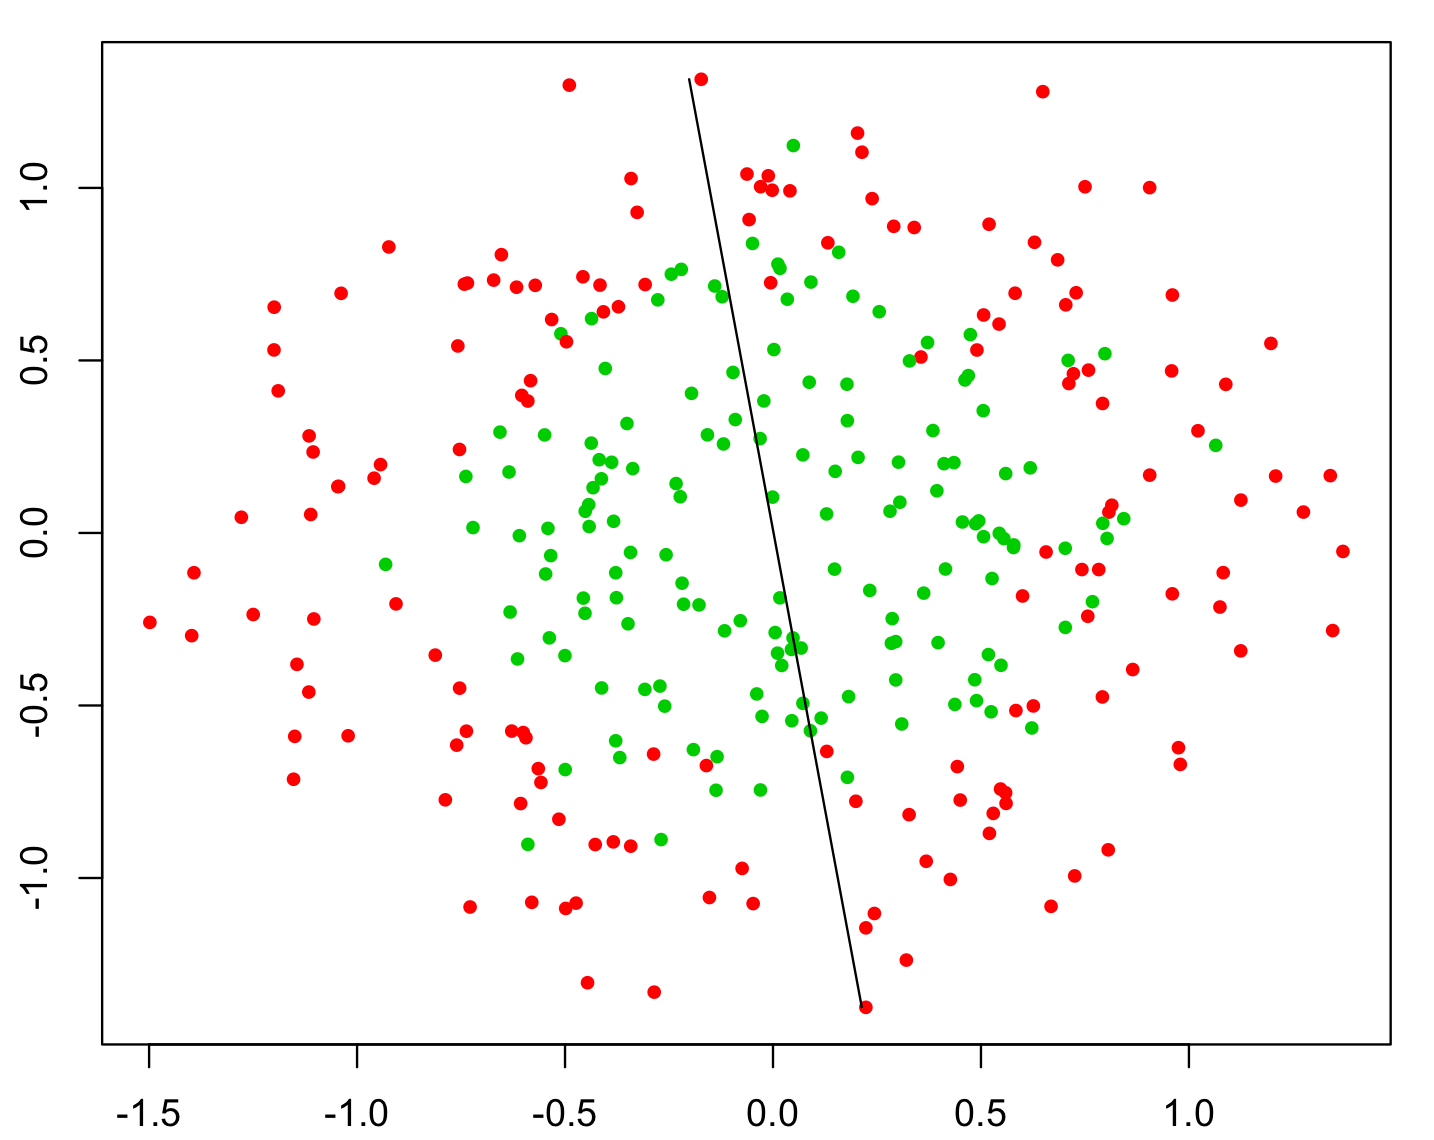
\includegraphics[height=4cm]{linear}
    \caption{Example of a linear activation function on non linearly separable data
    https://www.r-bloggers.com/interactive-visualization-of-non-linear-logistic-regression-decision-boundaries-with-shiny/}
\end{figure}

\begin{table}
    \caption{Table captions should be placed above the
    tables.}\label{tab1}
    \begin{tabular}{|l|l|l|}
    \hline
    Function name &  Formule & Graph\\
    \hline
    Title (centered) &  {\Large\bfseries Lecture Notes} & lol \\
    1st-level heading &  {\large\bfseries 1 Introduction} & 12 point, bold\\
    2nd-level heading & {\bfseries 2.1 Printing Area} & 10 point, bold\\
    3rd-level heading & {\bfseries Run-in Heading in Bold.} Text follows & 10 point, bold\\
    4th-level heading & {\itshape Lowest Level Heading.} Text follows & 10 point, italic\\
    \hline
    \end{tabular}
\end{table}




\begin{figure}
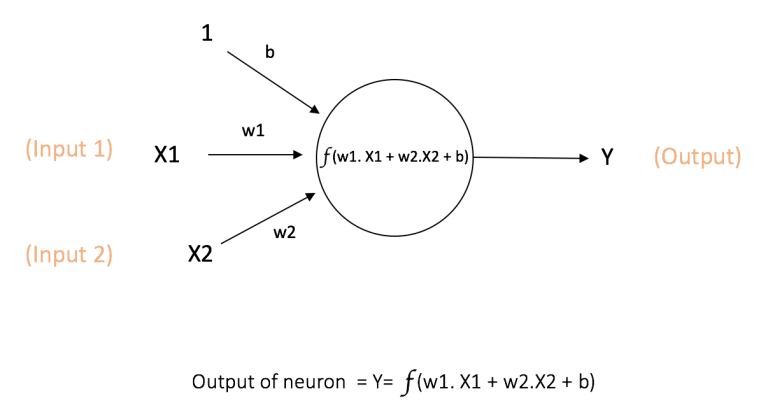
\includegraphics[height=6cm]{neuron}
\caption{https://ujjwalkarn.me/2016/08/09/quick-intro-neural-networks/}
\end{figure}
%
% ---- Bibliography ----
%
% BibTeX users should specify bibliography style 'splncs04'.
% References will then be sorted and formatted in the correct style.
%
% \bibliographystyle{splncs04}
% \bibliography{mybibliography}
%
\begin{thebibliography}{8}
\bibitem{ref_article1}
Author, F.: Article title. Journal \textbf{2}(5), 99--110 (2016)

\bibitem{ref_lncs1}
Author, F., Author, S.: Title of a proceedings paper. In: Editor,
F., Editor, S. (eds.) CONFERENCE 2016, LNCS, vol. 9999, pp. 1--13.
Springer, Heidelberg (2016). \doi{10.10007/1234567890}

\bibitem{ref_book1}
Author, F., Author, S., Author, T.: Book title. 2nd edn. Publisher,
Location (1999)

\bibitem{ref_proc1}
Author, A.-B.: Contribution title. In: 9th International Proceedings
on Proceedings, pp. 1--2. Publisher, Location (2010)

\bibitem{ref_url1}
LNCS Homepage, \url{http://www.springer.com/lncs}. Last accessed 4
Oct 2017
\end{thebibliography}
\end{document}
